\chapter{Opis modela}

\section{Konvolucijska neuronska mreža}

Konvolucijski modeli su prikladni za obradu podataka kod kojih nam je bitno ostvariti kovarijantnost na translaciju, primjerice slike kod kojih se isti objekt može pojaviti na više lokacija u slici. Naime, obični potpuno povezani modeli bi morali ponovno učiti za svaku moguću lokaciju objekta, što bi dovelo do loše generalizacije. Osim toga, za veće slike, potpuno povezani modeli bi zahtijevali preveliku količinu parametara.

Konvolucijski slojevi rješavaju ove probleme uvođenjem jezgri, koje za svoj izlaz razmatraju samo malo lokalno susjedstvo ulaza, koje potom "kližu" po ulazu te grade mapu značajki na ulazu. Nadalje, sažimanjem se postupno smanjuje veličina ulaza u svaki sljedeći sloj, te se na kraju opet dolazi do potpuno povezanih slojeva.

\section{ResNet-18}

Duboka rezidualna mreža (ResNet) je vrsta konvolucijskih neuronskih mreža. Glavno obilježje rezidualnih mreža je postojanje preskočnih veza. Njihova uloga je da u sljedeći blok prenose ulaz trenutnog bloka, koji nije bio transformiran prolaskom kroz slojeve prošlog bloka. Model ResNet-18 je građen od 5 rezidualnih blokova. Svaki blok sadrži 3 konvolucijska sloja.

\noindent\\Rezidualni blok se može opisati sljedećim izrazima:

\[y_{l} = h(x_{l}) + F(x_{l}, W_{l})\]
\[x_{l+1} = f(y_{l}),\]
gdje su \(x_{l}\) i \(x_{l+1}\) ulaz i izlaz \(l\)-tog bloka, a \(F\) rezidualna funkcija. \(h(x_{l})\) je funkcija identiteta koja prenosi netransformirani ulaz u rezidualni blok. Rezidualna funkcija \(F\) je implementirana kao niz transformacija nad ulaznim podacima. Ulazni podaci se transformiraju prolaskom kroz konvolucijske slojeve bloka.

Kod detekcije objekta ResNet modelom, bitno je napomenuti da model nije osjetljiv na položaj tog objekta na slici. Na izlasku iz zadnjeg sloja odvija se average pooling. Average pooling uzima prosjek iz trenutnih vrijednosti u jezgri i sprema ga u mapu značajki. Objekt može biti na bilo kojem položaju na slici i uvijek dati istu mapu značajki.

\begin{figure}[h]
	\centering{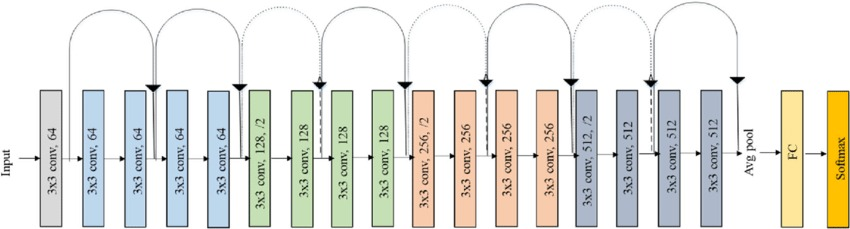
\includegraphics[scale=0.5]{slike/resnet.jpg}}
	\caption{Prikaz ResNet arhitekture}
	\label{resnet}
\end{figure}